\subsection{Erste Datensammlung und manuelle Aufbereitung}
Für eine möglichst gute Datengrundlage wurde an einer geraden Straße Aufnahmen von insgesamt 21 vorbeifahrenden Kfz gemacht, sowohl von dicht aufeinanderfolgenden, als auch einzelnen Fahrzeugen. Als Aufnahmegerät wurde ein Smartphone mit integrierter Rekorder-App verwendet. Die zusammenhängende Aufnahme aller Fahrzeuge wurde anschließend von Hand in einzelne Abschnitte unterteilt und als WAV-Audiodateien gespeichert. \draftred{Dieses unkomprimierte Format wurde gewählt, um die Implementierung der Datenanalyse zu erleichtern.}\todo[inline]{Andere Begründung?} %todo

\subsection{Analyse der Audiodaten via Dopplereffekt}
Da im Phy\-sik-Unter\-richt eine Abituraufgabe zur Geschwindigkeitsbestimmung eines Rennwagens mittels Differenz der Frequenz bei Annäherung und Entfernung behandelt wurde, ist das der erste verfolgte Ansatz. Es erscheint zudem einfach, die Geschwindigkeit akkurat zu ermitteln, da selbst ein Mensch eindeutige Frequenzveränderungen hören kann, beispielsweise bei einem vorbeifahrenden Krankenwagen mit Martinshorn. Allerdings muss bei normalen Kfz das Reifengeräusch anstelle des Martinshorns verwendet werden, da dieses mit Abstand die lauteste Geräuschquelle des Straßenverkehrs ist.

Wenn der Abstand des vorbeifahrenden Fahrzeugs zum Beobachter vernachlässigt und von konstanter Bewegungsgeschwindigkeit ausgegangen wird, können folgende Formeln zur Berechnung der Geschwindigkeit verwendet werden:

\[
    f_{1} = f_{0} * \frac{c}{c - v}
    \quad\text{und}\quad
    f_{2} = f_{0} * \frac{c}{c + v}
\]

Dabei ist \(f_{1}\) die vom Beobachter registrierte Frequenz bei Annäherung und \(f_{2}\) die Frequenz bei Entfernung des Fahrzeugs. Die Konstante \(c\) wird mit \(c = 343\frac{m}{s}\) als Schallgeschwindigkeit in Luft angenommen. Durch Messung beider Frequenzen kann das Frequenzverhältnis \(k = \frac{f_{1}}{f_{2}}\) berechnet und nach \(v\) umgestellt werden:

\begin{equation*}
    \begin{split}
        k & = \frac{f_{0} * \frac{c}{c - v}}{f_{0} * \frac{c}{c + v}} \\
        k & = \frac{c + v}{c - v} \\
        & \Leftrightarrow \\
        v & = \frac{k - 1}{k + 1} * c
    \end{split}
\end{equation*}

\begin{figure}[h]
    \centering
    \import{rsc/plots/f-t-plot/}{frequenz-zeit-plot.tex}
    \caption{Beispielhafter Frequenzverlauf bei vorbeifahrendem Fahrzeug}
    \label{fig:frequencyplot}
\end{figure}

Des Weiteren ist mit dem Dopplereffekt die Entfernungsbestimmung von Mikrofon und Fahrzeug möglich, indem die Änderungsgeschwindigkeit der Frequenz analysiert wird. Hierbei gilt: je größer die Änderungsrate, desto dichter sind Fahrzeug und Beobachter (siehe \autoref{fig:frequencyplot}).

\subsubsection{Verwendung der Reifengeräusche}

Für einen ersten Überblick wurden die Audio-Abschnitte in einen Spektrumanalysator geladen. Die Ergebnisse der visuellen Analyse sind in \autoref{img:spectrumanalyzer} dargestellt.

\begin{figure}[h]
    \begin{subfigure}{.5\textwidth}
        \centering
        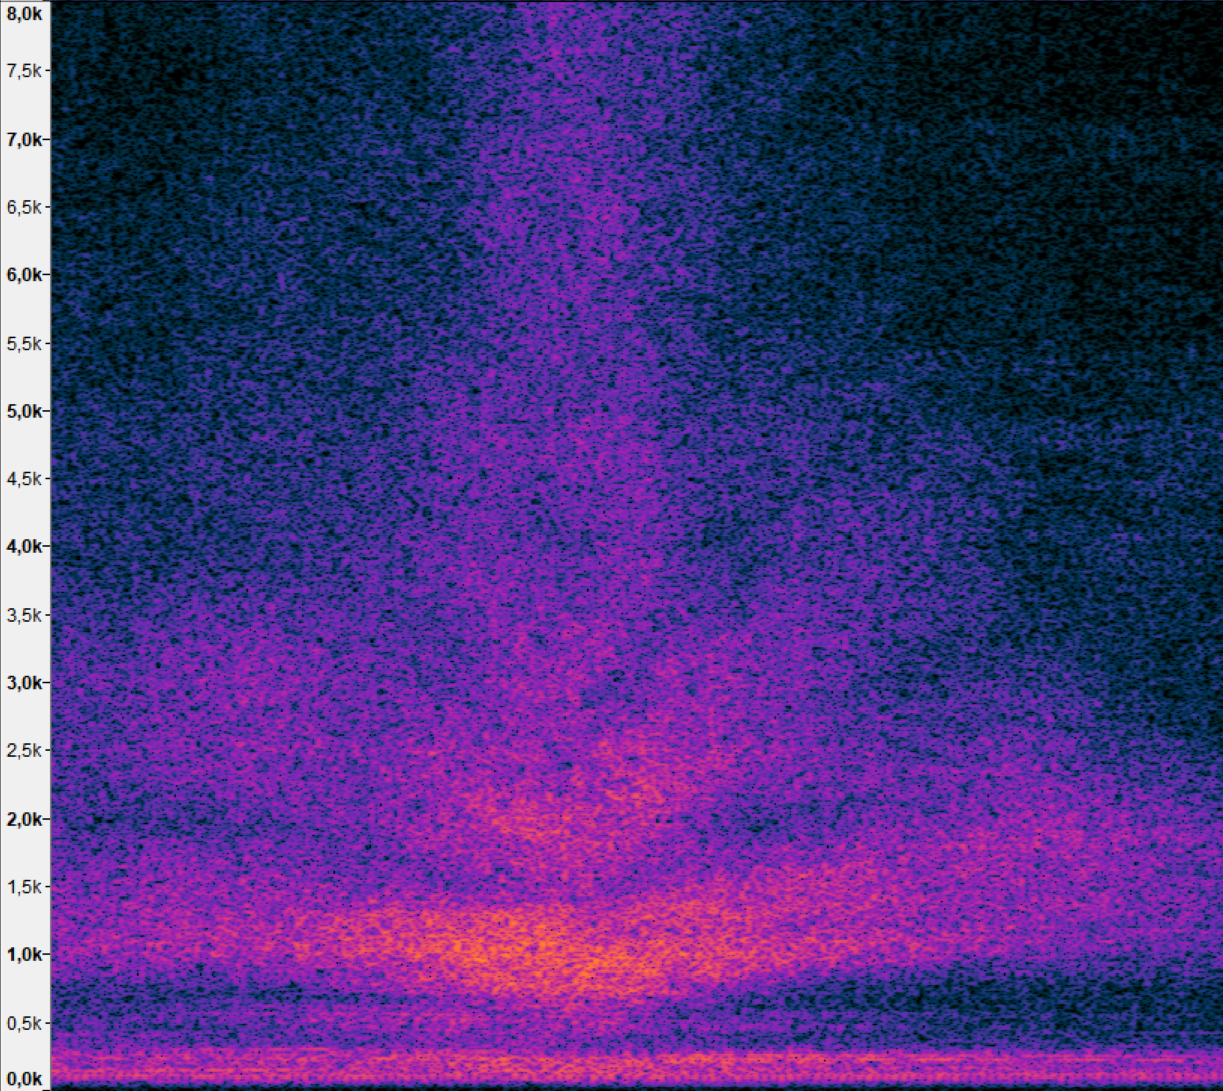
\includegraphics[width=.8\linewidth]{Frequenzen}
        \caption{Spektrogramm}
    \end{subfigure}
    \begin{subfigure}{.5\textwidth}
        \centering
        \includegraphics[width=.8\linewidth]{Tonhöhe(EAC)}
        \caption{Tonhöhe (EAC)}
        \label{img:spectrum_b}
    \end{subfigure}
    \caption{Ergebnisse Spektrumanalysator Reifengeräusche}
    \label{img:spectrumanalyzer}
\end{figure}

\autoref{img:spectrum_b} wurde nachbearbeitet. Die pinkfarbene Linie zeigt den Verlauf der Tonhöhe über Zeit und kann als Frequenzgraph interpretiert werden. Ab der tiefsten Stelle des Graphen ist das vorbeifahrende Kfz am nächsten zum Mikrofon.

Beim Vergleich mit einem theoretisch berechneten Frequenzgraph (\autoref{fig:frequencyplot}) fällt auf, dass die aufgenommene Frequenz der Reifengeräusche vor Vorbeifahren (in der Beispielabbildung bei \(t = 10 s\)) nicht höher ist als nach dem Vorbeifahren, sondern bei niedrigerem Abstand geringer ist. Es konnte keine wissenschaftliche Erarbeitung dieses Phänomens gefunden werden, am wahrscheinlichsten ist jedoch eine Reflexion der akustischen Wellen am Boden, die mit den direkt zum Mikrofon laufenden Wellen interferieren und somit hohe Frequenzen auslöschen. Aufgrund dieser unklaren Messergebnisse kann dieser Ansatz jedoch nicht weiterverfolgt werden.

\subsubsection{Verwendung der Motorgeräusche}

\begin{figure}[h]
    \centering
    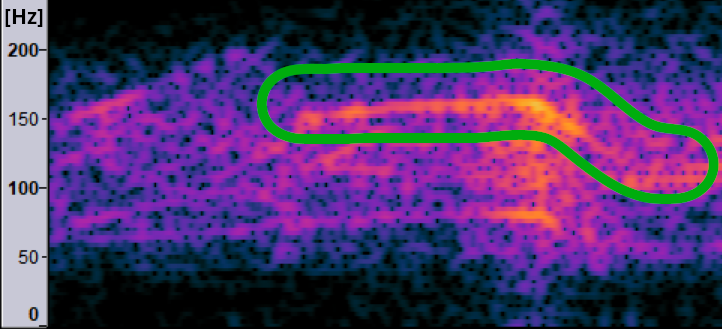
\includegraphics[width=.6\linewidth]{SpektrogrammMotor}
    \caption{Spektrogramm Motorgeräusche}
    \label{fig:spectrum_motor}
\end{figure}

Nachdem sich die Reifengeräusche als unbrauchbar erwiesen haben, ist nun der nächste Ansatz, die Motorgeräusche aufgrund der eindeutigeren Tonhöhe -- anstatt eines Rauschens -- zu analysieren. Hierfür wird ein Tiefpass mit einer Grenze von \(150 Hz\) auf die Audiospur gelegt, um Reifengeräusche möglichst gut herauszufiltern. Bei der manuellen Analyse stellt sich jedoch heraus, dass selbst die besten Aufnahmen unbrauchbar sind: Der in \autoref{fig:spectrum_motor} grün umrandete Frequenzverlauf stellt die aufgenommenen Motorgeräusche dar, bei denen die Dopplerverschiebung sichtbar ist. Zwar beinhaltet die Aufnahme vor dem Vorbeifahren des Kfz eindeutige Motorgeräusche, allerdings gibt es keine Messpunkte bei Entfernung des Fahrzeugs (hinter dem „Knick“ im Spektrogramm verschwindet die helle, gelbe Linie). Die Motorgeräusche, die direkt mit der Motordrehzahl zusammenhängen, konnten vom verwendeten Handymikrofon gar nicht aufgezeichnet werden, vermutlich unterläge es jedoch den gleichen Einschränkungen wie die aufgezeichneten Oberwellen. Somit kann auch diese Variante der Geschwindigkeitsbestimmung nicht verwendet werden.

\subsection{Analyse der Audiodaten via Lautstärkeänderung}
Für eine Berechnung der Geschwindigkeit von Fahrzeugen anhand ihrer Lautstärke muss das Verhältnis zwischen Lautstärke und Abstand bekannt sein. Dieses wird im folgenden Versuch experimentell erforscht. Die empirischen Ergebnisse werden anschließend mit einer mathematischen Beziehung verglichen.

Für eine Berechnung der Geschwindigkeit von Fahrzeugen anhand ihrer Lautstärke muss das Verhältnis zwischen Lautstärke und Abstand bekannt sein. Die ausschlaggebende Größe für die „Lautstärke“ ist der Schalldruck \(p\), der umgekehrt proportional zur Entfernung ist:
\[
    p \sim \frac{1}{r}
\]

Da der Schalldruck mit einem herkömmlichen Mikrofon jedoch nicht gemessen werden kann, muss eine Umrechnung der aufgenommenen Amplitude auf den Schalldruckpegel (umgangssprachlich oft als „Schallpegel“ bezeichnet) vorgenommen werden. \footcite{SchalldruckMessen}
Da ein Pegel immer eine relative Größe ist, wurde als Referenzwert die maximal von einer Audiodatei speicherbare Amplitude gewählt. Die Gesetzmäßigkeit, dass sich der Schallpegel pro Abstandsverdoppelung um \(6 dB\) verkleinert, wird reziprokes Abstandsgesetz genannt \footcite{SengpielSchallpegelEntfernung} und kann in die Formel
\[
    L_{2} = L_{1} - \abs{20 * \log{\left(\frac{r_{1}}{r_{2}}\right)}}
\]
übertragen werden. \(L\) ist hierbei der Schallpegel in \(dB\), \([r] = 1 m\) ist der Abstand von Schallquelle und Schallempfänger. \footcite{SengpielSchallpegelEntfernung} Mit den Indizes \(1, 2\) sind erster und zweiter Messpunkt gekennzeichnet (siehe auch \autoref{img:SchalldruckpegelSymbolbild}). Durch Umformung nach \(r_{2}\) erhält man
\begin{equation}
    \begin{split}
        r_{2} = r_{1} * 10^{\left(\frac{\abs{L_{1} - L_{2}}}{20}\right)} \\
        d_{2} = \sqrt{r_{2}^2 - d_{a}^2}
    \end{split}
    \label{formula:RadiusAusSchallpegel}
\end{equation}
womit sich bei bekannter Zeitspanne zwischen der ersten und der zweiten Messung unter Berücksichtigung von Pythagoras die Geschwindigkeit des vorbeifahrenden Fahrzeugs bestimmen lässt:
\[
    v = \frac{d_{2} - d_{1}}{\Delta t_{1,2}}
\]

\begin{figure}[h]
    \centering
    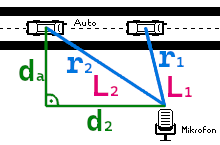
\includegraphics[width=.4\linewidth]{SchalldruckpegelSymbolbild}
    \caption{Symbolbild Schalldruckpegel und Abstand (\(d_{a}\): Abstand zur Straße)}
    \label{img:SchalldruckpegelSymbolbild}
\end{figure}

Wenn \(d_{a}\) jedoch unbekannt ist, kann keine Geschwindigkeitsberechnung vorgenommen werden, selbst bei der Annahme, dass der Abstand des Mikrofons zur Straße vernachlässigbar ist (\(d_{a} \approx 0\)).

Dieses Problem kann an folgendem Gedankenexperiment veranschaulicht werden: Eine Schalldruckpegel-Änderung um \(+6 dB\) kann interpretiert werden als ein Fahrzeug,
\begin{enumerate}
    \item welches sich von \(200 m\) zu \(100 m\) Entfernung (\(100 m\) Entfernungsunterschied) innerhalb der Zeit \(\Delta t\) angenähert hat.
    \item welches sich von \(100 m\) zu \(50 m\) Entfernung (\(50 m\) Entfernungsunterschied) innerhalb der gleichen Zeit \(\Delta t\) angenähert hat.
\end{enumerate}
Dies hätte zur Folge, dass für das Fahrzeug aus Beispiel \((1)\) die doppelte Geschwindigkeit \(v\) wie für Fahrzeug \((2)\) berechnet würde, da es keinen Referenzwert gibt.

Bei bekanntem Abstand zur Straße kann die Aufnahme auf Hochpunkte im Schalldruckpegel untersucht werden. Der Hochpunkt stellt dann den Moment der geringsten Distanz zwischen Mikrofon und Fahrzeug dar. Damit wird die Unbekannte \(r_{1}\) in \autoref{formula:RadiusAusSchallpegel} durch \(d_{a}\) ersetzt und die Unbekannte ist eliminiert. Durch eine Normalisierung der Audiorohdaten auf \(-0 dB\) kann dann für \(L_{1}\) selbiger Gleichung \(L_{1} = 0 [dB]\) eingesetzt werden, was eine weitere Unbekannte eliminiert. Nun muss lediglich der Schalldruckpegel \(L_{2}\) aus den Audiodaten berechnet werden, um den Abstand \(r_{2}\) zu ermitteln.


\subsubsection{Versuch zur Bestimmung der Beziehung zwischen Lautstärke und Abstand}

\begin{figure}[h]
    \begin{subfigure}{.5\textwidth}
        \centering
        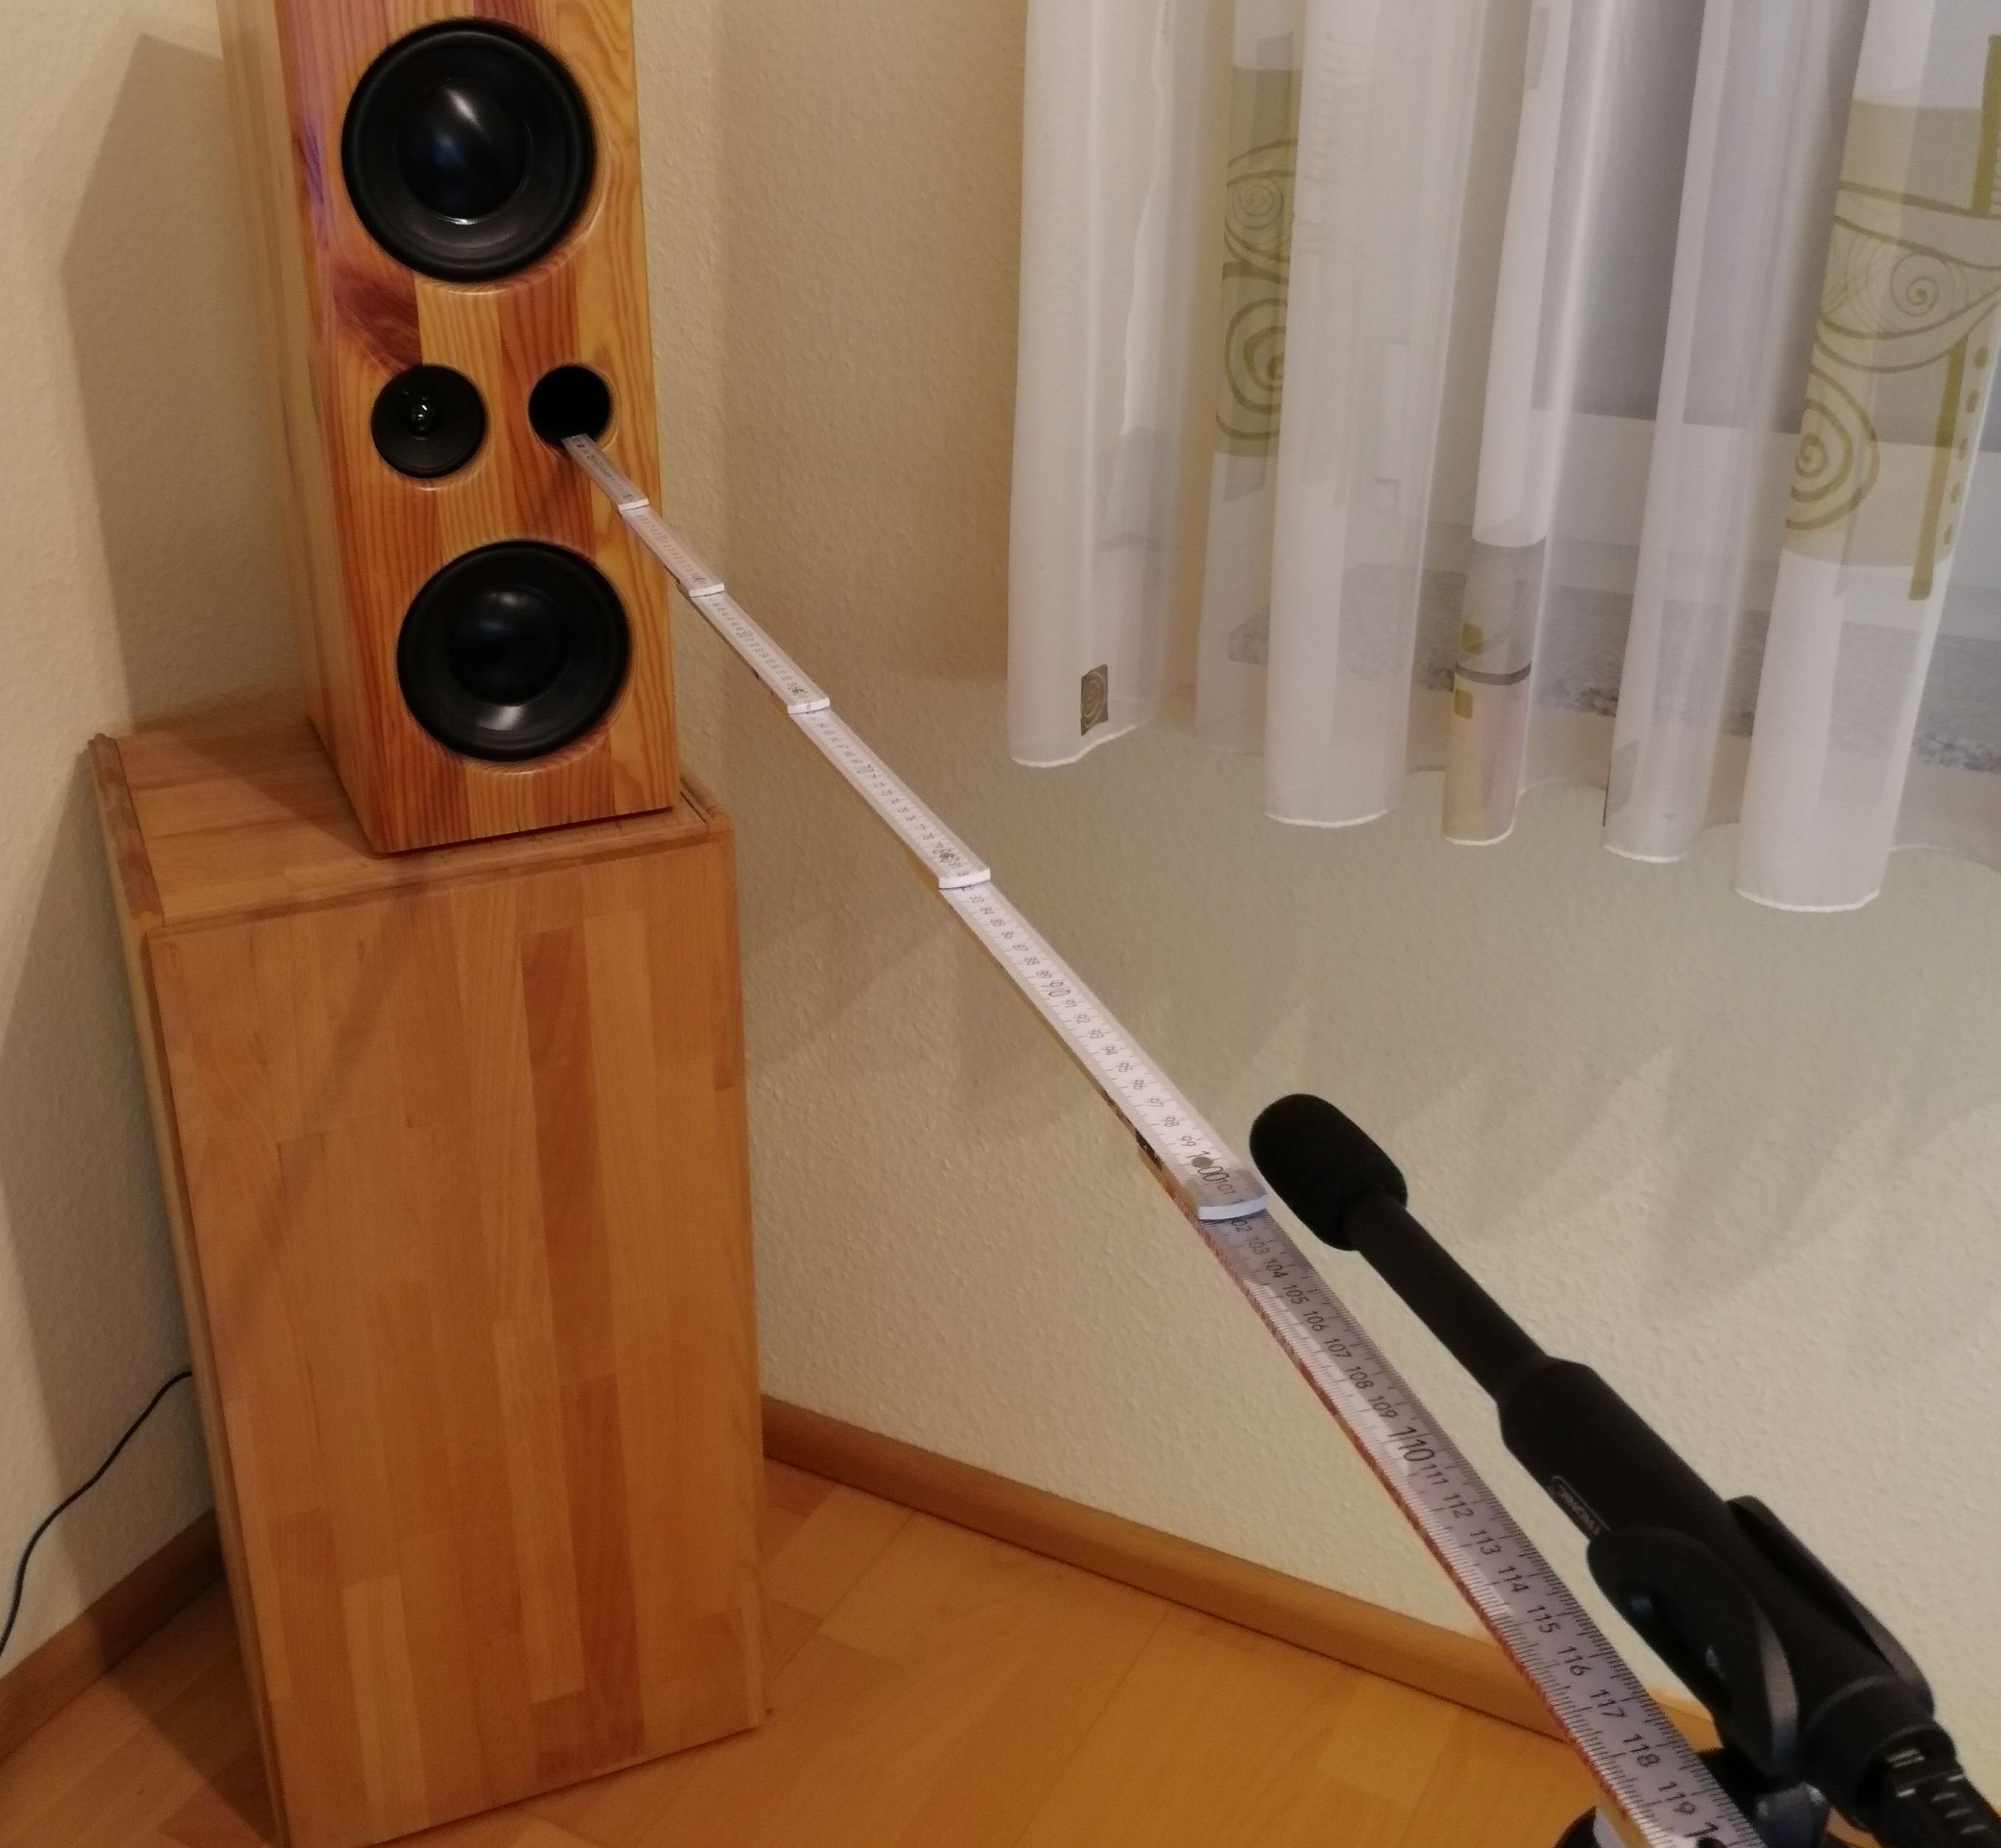
\includegraphics[width=.8\linewidth]{VersuchsaufbauAbstandInnen}
        \caption{Innenraum}
        \label{img:dist_room}
    \end{subfigure}
    \begin{subfigure}{.5\textwidth}
        \centering
        \includegraphics[width=.95\linewidth]{VersuchsaufbauAbstandsmessung}
        \caption{Im Freien}
        \label{img:dist_free_field}
    \end{subfigure}
    \caption{Versuchsaufbau zur Lautstärkebestimmung}
    \label{img:versuche_abstand}
\end{figure}

Zuerst wurde eine Messreihe zum Verhältnis zwischen Lautstärke und Abstand im Innenraum durchgeführt. Hierfür wurde ein im Eck stehender Lautsprecher und ein Messmikrofon auf einem Stativ gegenübergestellt (siehe \autoref{img:dist_room}). Bei verschiedenen Abständen wurde zunächst ein \(1 kHz\)-Ton über den Lautsprecher abgespielt und vom Mikrofon aufgenommen. Bei der Auswertung der Messergebnisse stellte sich heraus, dass der Innenraum bei bestimmten Abständen die Töne „verschluckt“, da durch Reflexionen der Schallwelle an den Innenwänden des Raumes an diesen Punkten eine destruktive Interferenz entsteht. Da das Interferenzmuster von der Frequenz der Schallwelle abhängt, wurde anschließend der gleiche Versuch mit einem weißen Rauschen als ausgesendetes Geräusch verwendet, um durch das breite Frequenzspektrum die Tiefpunkte der Lautstärke zu vermeiden. Zur Berechnung des effektiven Schalldruckpegels wurde das Programm „Audacity“ \footcite{Audacity} und dessen „Measure RMS“-Funktion verwendet.

Bei der Auswertung der Aufnahmen stellte sich heraus, dass für Abstandsverdoppelung der Schalldruckpegel um etwa \(4 dB\) absank, was nur zwei Drittel der erwarteten Absenkung entspricht. Diese Abweichung lässt sich auf den Versuchsaufbau zurückführen: Der Lautsprecher stellt in seiner aktuellen Aufstellung eine gerichtete Schallquelle dar, der verwendete Innenraum ist nicht reflexionsarm. Beides sind Ausschlusskriterien für die Anwendbarkeit des reziproken Abstandsgesetzes, da der Pegelabfall dadurch geringer ausfällt.

Um beide Probleme zu beheben, wurde ein zweiter Versuch durchgeführt. Dieser fand im Freien statt, um Reflexionen an Wänden zu vermeiden. Zudem wurde der verwendete Lautsprecher mit seiner Membran (Chassis) nach oben ausgerichtet, das Mikrofon wurde für die Entfernungsmessung jedoch weiterhin in der Horizontalen bewegt. Somit kann die Schallquelle näherungsweise als Quelle mit kugel- bzw. halbkugelförmiger Charakteristik betrachtet werden, ähnlich wie es ein vorbeifahrendes Fahrzeug darstellt. Es wurden drei Messreihen aufgestellt, die ersten beiden davon mit gleicher Ausgabeamplitude des Lautsprechers, die dritte mit geringerer Amplitude.

\begin{figure}[h]
    \begin{subfigure}{.5\textwidth}
        \centering
        \import{rsc/plots/d-L-plot/}{abstand-pegel-plot.tex}
        \caption{Rohdaten}
        \label{fig:pegelplot_roh}
    \end{subfigure}
    \hfil
    \begin{subfigure}{.5\textwidth}
        \centering
        \import{rsc/plots/d-L-plot/}{d-L-avg-plot.tex}
        \caption{Mittelwert und Vergleichsfunktion}
        \label{fig:pegelplot_avg}
    \end{subfigure}
\end{figure}

In \autoref{fig:pegelplot_roh} sind die aufgenommenen Rohdaten aller Messreihen. Diese werden in \autoref{fig:pegelplot_avg} mit der Logarithmus-Funktion für den Bezug von Schalldruckpegel und Distanz verglichen. Es fällt auf, dass die gemittelte Pegelfunktion fast identisch mit der Logarithmus-Funktion ist, wodurch der Zusammenhang der Pegelabnahme um sechs Dezibel pro Abstandsverdoppelung bestätigt.


http://www.sengpielaudio.com/Rechner-entfernung.htm

http://www.sengpielaudio.com/Rechner-abstandsgesetz.htm